%\documentclass{standalone}
%\usepackage{fontspec}
%\usepackage{polyglossia}
%\usepackage{tikz}
%\usepackage{ifthen}    
%\usepackage{tikz-3dplot}
%%
%\setmainlanguage{english}
%\setotherlanguages{arabic}
%\newfontfamily\arabicfont[Scale=1.0,Script=Arabic]{Scheherazade}
%\newfontfamily\urdufont[Scale=1.0,Script=Arabic]{XB Tabriz}
%%
%\begin{document}
%\begin{urdufont}
\tikzsetnextfilename{figVectors/figVectorHeadToTailRule}
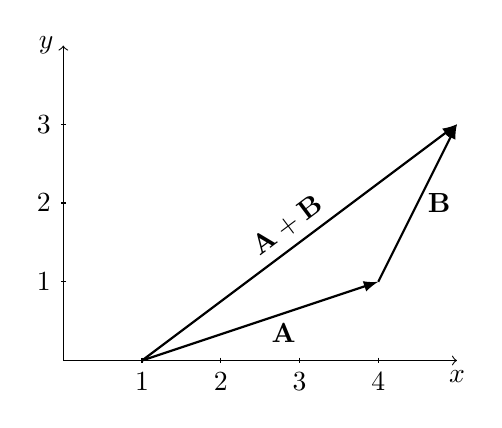
\begin{tikzpicture}
%\draw[help lines, thick] (0,0) grid (5,4);
\draw[<->] (0,4)--(0,0)--(5,0);
\node[left] at (0,4) {$y$};
\node[below] at (5,0) {$x$};
\draw[thick, -latex] (1,0)--(4,1) node[pos=0.6,below]{$\bf{A}$};
\draw[thick, -latex] (4,1)--(5,3)node[pos=0.5,right]{$\bf{B}$};;
\draw[thick, -latex] (1,0)--(5,3) node[pos=0.5,sloped, above]{$\bf{A+B}$} ;
%
\foreach \x/\xl in {1/1,2/2,3/3,4/4}
\draw (\x,1pt) --(\x,-1pt) node [anchor=north] {$\xl$};
\foreach \y in {1,2,3}
\draw (+1pt,\y) --(-1pt,\y) node [anchor=east] {$\y$};
\end{tikzpicture}
%\end{urdufont}
%\end{document}
